\subsection{Транзакции. Восстановление. Классический алгоритм}

\subsubsection{Транзакции}

\begin{definition}
    \textit{Транзакция} -- минимальный объем работы, который можно
    зафиксировать в базе данных.
\end{definition}

Каждый оператор заключен в неявную транзакцию, которая начинается
непосредственно перед оператором и заканчивается после него.
Не все действия в СУБД являются транзакционными.
Например, во многих реализациях не поддерживается транзакционное изменение
схемы данных.

\paragraph{Свойства транзакций (ACID)}

\begin{definition}
    \textit{Атомарность (Atomicity)} -- с точки зрения БД, транзакция либо
    выполняется целиком, либо полностью откатывается. Иначе говоря, никто
    со стороны не может увидеть промежуточное состояние выполнения транзакции.
\end{definition}

\begin{definition}
    \textit{Согласованность (Consistency)} -- после завершения транзакции БД
    остается в согласованном состоянии.
\end{definition}

\begin{definition}
    \textit{Изоляция (Isolation)} -- транзакции не могут взаимодействовать
    между собой. Это означает, что транзакции не могут пользоваться
    промежуточными результатами друг друга.
\end{definition}

\begin{definition}
    \textit{Устойчивость (Durability)} -- при успешном завершении транзакции
    результаты ее исполнения сохраняются в БД, при откате транзакции все
    внесенные ею изменения отменяются.
\end{definition}

\paragraph{Корретность и согласованность}

\begin{definition}
    Состояние БД является \textit{согласованным}, если оно удовлетворяет всем
    объявленным ограничениям. Это свойство автоматически проверяется СУБД.
\end{definition}

\begin{definition}
    Состояние БД является \textit{корректным}, если оно соответствует реальному
    миру. Автоматически проверено быть не может.
\end{definition}

Существуют условия корректности, которые нельзя проверить ограничениями.
Например, после перевода денег в банке их общая сумма в системе не должна
измениться. Однако, эта сумма заранее неизвестна, поэтому заранее задать
ограничение невозможно.

\paragraph{Минимизация транзакций}

Транзакции требуют большие ресурсные затраты, поэтому должны быть минимальными.
По возможности следует использовать неявные транзакции.

Однако, есть типичные ситуации, в которых использования неявных транзакций
недостаточно:

\begin {itemize}
    \item \textit{Условное обновление} -- проверку условия и обновление
        необходимо сделать в рамках одной транзакции, в противном случае в
        момент изменения условие может перестать выполняться;
    \item \textit{Множественное обновление} -- при обновлении данных, особенно
        в различных таблицах, использование транзакции необходимо для
        исключения несогласованности;
    \item \textit{Промежуточная несовместимость} -- некоторые действия требуют
        временного нарушения согласованности с последующим его восстановлением,
        использование транзакций позволяет откладывать проверку согласованности
        до завершения всех действий и исключают видимость несогласованного
        состояния другими пользователями.
\end {itemize}

Также следует отметить, что результат завершения транзакции
\textbf{не должен зависеть от человека}. Человеческий фактор может привести к
зависшей транзакции. Если требуется принятие решения от человека, транзакцию
следует разбить на две: первая читает данные, а вторая их записывает,
предварительно проверяя данные на соответствие результату первой. В таком
случае от решения человека зависит применение второй транзакции.

\subsubsection{Восстановление}

Напомним, что свойство \textit{устойчивости (durability)} транзакции
подразумевает сохранение результатов транзакции в БД даже при сбоях.

Хранение данных в оперативной памяти может приводить к потерям, например, при
перезагрузке. Это считается нормальным, что приводит к необходимости хранения
информации на дисках. Напомним, что с диска быстрее читать данные
последовательно.

\paragraph{Типы сбоев}

\begin{itemize}
    \item \textbf{Локальный}. Сбой одной транзакции. Для восстановления
        достаточно откатить затронутую транзакцию.
    \item \textbf{Глобальный}. Сбой процесса СУБД, затрагивает все транзакции.
        Для восстановления достаточно откатить все незавершенные транзакции, а
        также заново применить все успешно завершенные транзакции.
    \item \textbf{Аппаратный}. Например, перезагрузка компьютера. С точки
        зрения СУБД, не существенно отличается от глобального сбоя.
    \item \textbf{Отказ оборудования}. СУБД не может восстановиться после этого
        типа сбоя. Однако, многие СУБД предоставляют \textit{средства}
        для восстановления (например, запись данных на несколько дисков и
        синхронизация копий).
\end{itemize}

Свойство устойчивости не является абсолютным. Существуют сбои, при которых его
нельзя поддержать.

\paragraph{Восстановление после сбоя}

Для восстановления БД достаточно сделать следующее:

\begin{itemize}
    \item Успешные транзакции -- зафиксировать;
    \item Откаченные транзакции -- откатить;
    \item Незавершенные транзакции -- откатить.
\end{itemize}

Существует несколько популярных подходов для отката:

\paragraph{Shadow copy}

Каждая транзакция пишет данные в новое место. При успешном завершении
транзакции копия помечается успешной, пользователь уведомляется об успешной
транзакции, и начинается запись из копии в БД. При сбое во время записи
производится повторная запись. Проблема подхода заключается в частых чтениях и
записях shadow copy, которые расположены в случайных местах на диске, что
медленно.

\paragraph{Transaction log}

Данные пишутся сразу в БД, параллельно записывая изменения, примененные в
рамках каждой транзакции, в журнал. Данный подход более популярен.

Журнал записывается в надежное хранилище изменений. Это означает,
что его утрата есть невосстановимый сбой. Однако, записи ведутся
последовательно, что делает данный подход быстрее предыдущего.

В журнал записываются: старые данные, новые данные, маркеры начала и завершения
транзакции.

При завершении транзакции все изменения записываются в журнал, записывается
маркер завершения транзакции, пользователь уведомляется о завершении
транзакции.

\paragraph{Реализация журнала}

\begin{itemize}
    \item \textbf{Постоянная запись на диск}. При записи каждого изменения в
        журнал существенно возрастает число операций, конкуренция за доступ к
        диску, а также накапливаются откаченные транзакции, которые в будущем
        не принесут пользы.
    \item \textbf{Запись при завершении}. В журнал при завершении транзакции
        записываются порожденные изменения. При больших изменениях это приводит
        к росту потребления памяти журналом.
    \item \textbf{Точки восстановления}. В журнал периодически записывается
        "слепок" состояния системы: текущие изменения, завершенные транзакции
        (не записанные ранее), откаченные транзакции (не записанные ранее),
        открытые транзакции. Создание точки восстановления требует приостановки
        изменений.
\end{itemize}

\paragraph{Структура журнала}

С использованием механизма точек восстановления, получаем следующую структуру
журнала.

\begin{itemize}
    \item \textbf{Точка восстановления};
    \item \textbf{События}:
        \begin{itemize}
            \item Идентификатор транзакции,
            \item Указатель на \textit{предыдущее} событие транзакции:
                \begin{itemize}
                    \item Начало транзакции,
                    \item Изменение,
                    \item Завершение транзакции,
                    \item Откат транзакции.
                \end{itemize}
        \end{itemize}
\end{itemize}

\paragraph{Примеры}
Рассмотрим пример сбоя и определим, что должно произойти с каждой из транзакций.

\begin{figure}[h]
    \centering
    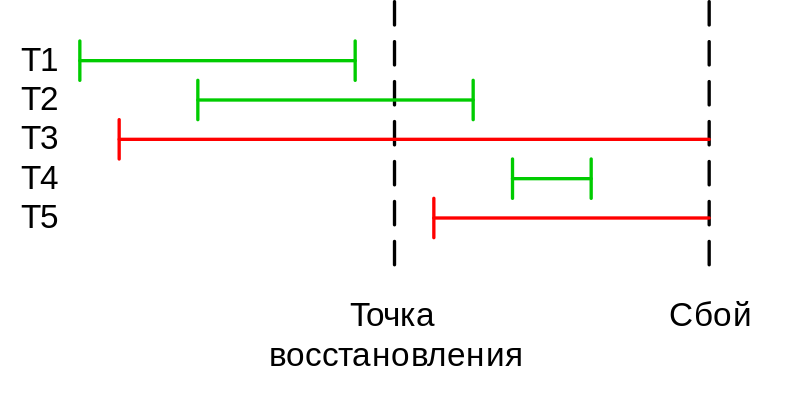
\includegraphics[width=0.8\textwidth]{../assets/kgeorgiy/transactions/Recovery_TransactionLog_2.svg.png}
    \caption{Иллюстрация к определению проекции}
    \label{tx-log}
\end{figure}

Зеленым и красным цветом отмечены транзакции, которые должны быть завершены или
откачены соответственно при восстановлении. Отметим, что эти решения однозначно
определены гарантиями ACID транзакций.

\subsubsection{Классический алгоритм восстановления}

\paragraph{Фазы алгоритма}

\begin{itemize}
    \item \textbf{Разметка транзакций}. Каждая транзакция отмечается как
        \textit{Redo} или \textit{Undo}.
    \item \textbf{Откат транзакций}. Для помеченных как \textit{Undo}.
    \item \textbf{Повтор транзакций}. Для помеченных как \textit{Redo}.
\end{itemize}

\paragraph{Фаза разметки транзакций}

\begin{itemize}
    \item Чтение журнала идет от последней точки восстановления до конца. Все
        открытые транзакции помещаются в \textit{Undo}.
    \item При чтении маркера начала транзакция добавляется в \textit{Undo}.
    \item При чтении маркера конца транзакция переносится из \textit{Undo} в
        \textit{Redo}.
\end{itemize}

\paragraph{Фаза повторения транзакций}

\begin{itemize}
    \item Чтение журнала идет от последней точки восстановления до конца.
    \item При чтении маркера конца транзакция удаляется из \textit{Redo}.
    \item При чтении изменения оно применяется, если транзакция в \textit{Redo}.
\end{itemize}

\begin{proposition}
    После успешного выполнения всех фаз БД находится в корректном состоянии и
    гарантирует выполнения свойства устойчивости.
\end{proposition}

\begin{proposition}
    Рассмотрим все открытые транзакции. Для каждой из них найдем ближайшую
    точку восстановления из будущего. Все данные до самой ранней точки
    восстановления из рассматриваемых можно удалить, поскольку они не
    понадобятся при восстановлении.
\end{proposition}
